\documentclass{article}
\usepackage[utf8]{inputenc}
\setlength{\parskip}{5pt} % esp. entre parrafos
\setlength{\parindent}{0pt} % esp. al inicio de un parrafo
\usepackage[spanish]{babel}
\usepackage[sort&compress,numbers]{natbib} % referencias
\usepackage[top=25mm,left=20mm,right=20mm,bottom=25mm]{geometry} % margenes
\usepackage{graphicx} % poner figuras
\usepackage{color,listings}
\usepackage{tikz}
\usepackage{minted}
\usetikzlibrary{automata,topaths}
\renewcommand\lstlistingname{Código}
\title{P2}
\author{Ismael Crespo}
\date{\today}
\begin{document}

\maketitle

\section{Introducción.}
Este trabajo presenta tres experimentos distintos donde se simula un autómata celular en dos dimensiones, la generación de vida a partir de semillas aleatorias, y finalmente un autómata celular en tres dimensiones. La programación se realizo en \emph{Python 3.10.2} y se utilizó la selección pseudoaleatoria de números como base para la simulación de cada caso.
\section{Objetivo.}
1.-Estudiar la probabilidad de vida en un autómata celular en 2 dimensiones después de un número determinado de pasos $n_p$, variando el número de elementos en la matriz $num$ y el valor mínimo para dejar vivas las celdas al inicio $p$.

2.-Modelar algún tipo de crecimiento o cristalización en la microestructura de un material. Núcleos aparecen al azar en celdas desocupadas y expanden con una tasa constante a celdas vecinas hasta agotar el espacio disponible. Examina la distribución de los tamaños de los núcleos que no toquen el borde al finalizar la simulación.

3.-Ejecutar un autómata celular en un modelo tridimensional.
 
\section{Programación en Python.}
Se realizaron tres códigos diferentes, la base en todos los casos es el uso de herramientas (\texttt{random}, \texttt{rand.int}, \texttt{random.choose}) que generan y seleccionan de manera pseudoaleatoria números para posicionar vida o semillas así como elegir las características de las semillas, como antecedentes se utilizó como base la lógica de programación presentada en trabajos previos por E.Schaeffer \citep{E.Schaeffer}.Véase referencia \citep{REPOP2} para consulta completa de los códigos.
\subsection {Autómata Celular en 2 dimensiones variando $n_p$ y $num$.}
Para comenzar con la simulación de un autómata celular se generaron valores con la herramienta \texttt{random} estos valores van desde $0.0$ a $1.0$ posteriormente el código elimina del vector de valores aquellos que sean menores a $p$, para finalizar, durante un determinado número de veces se analizan las vecindades de cada elemento, y aquellas donde a sus alrededores existan más de 3 elementos con vida, serán eliminaran. Para nuestros análisis el valor de $p$  tuvo valores de $0.2, 0.4, 0.6$ y $0.8$ y se hizo cada caso para matrices con $num$=$100, 225$ y $400$ (Código \ref{R1}).

Una vez terminado el experimento se encuentra la probabilidad de terminar con vida cada replica, por lo que se divide el número de replicas que tuvieron vida $R_v$al final entre el total de replicas $R_t$.
\begin{equation}
    Probabilidad=\frac{R_v}{R_t}*100
\end{equation}
\lstset{basicstyle=\ttfamily, keywordstyle=\bfseries}
\begin{lstlisting}[frame=single,numbers=left,language=Python,caption=Programación de un autómata celular variando el valor de $p$ y $num$\label{R1}]
  for d in (dim):
        xp=0
        for p in (p_value):
            num = d**2
            total=0
            for rep in range(replicas):
                valores = [1 * (random() < p) for i in range(num)]
                actual = np.reshape(valores, (d, d))
                def mapeo(pos):  
                    fila = pos // d
                    columna = pos % d
                    return actual[fila, columna]
                assert all([mapeo(x) == valores[x]  for x in range(num)])
                def paso(pos):
                    fila = pos // d
                    columna = pos % d
                    vecindad = actual[max(0, fila - 1):min(d, fila +2),
                       max(0, columna - 1):min(d, columna + 2)]
                    return 1 * (np.sum(vecindad) - actual[fila, columna] == 3)
                for iteracion in range(dur):
                    valores = [paso(x) for x in range(num)]
                    actual = np.reshape(valores, (d, d))
\end{lstlisting}  
\subsection{Simulación de un crecimiento o cristalización en una microestructura}
La simulación de un crecimiento se generó modificando el código \ref{R1}, de manera similar se utilizó la herramienta \texttt{random.choice} para colocar semillas de distintos valores, las semillas fueron colocadas un número determinado de veces y posteriormente se analizó cada elemento de la matriz que no tuviera valor para que seleccionara de manera pseudoaleatoria un valor que estuviera dentro de su vecindad, y así generar crecimientos hasta que todos los elementos tuvieran valores.
\subsection{Autómata tridimensional.}
El autómata tridimensional fue creado utilizando \texttt{matplotlib} para generar la gráfica de una matriz tridimensional y utilizando la lógica descrita en la sección 3.1 se eliminaron los elementos que estuvieran rodeados por más de 5 elementos en las tres dimensiones, dicho elementos fueron seleccionados de manera aleatoria para ser analizados por medio de la herramienta \texttt{random.choice} que selecciona un número pseudoaleatorio de matriz, columna y celda.
\section{Resultados.}
La figura \ref{prob} presenta la probabilidad, obtenida con la ecuación 1, de encontrar vida variando los valores de $p$ y de $num$ en un autómata celular, de esta gráfica podemos deducir que al existir mayores espacios que puedan ser ocupado por vida, las vecindades no están tan saturadas por lo que no se eliminarán tantas celdas con vida. El valor de $p$ nos indica que tan saturado va a estar cada matriz, a valores altos de $p$ naturalmente la población inicial va a ser alta y por lo tanto existe menos posibilidad de vida (figura \ref{p0.8}). Encontramos un valor óptimo cuando $p=0.4$ en una matriz de $num=400$.
\begin{figure} 
    \centering
    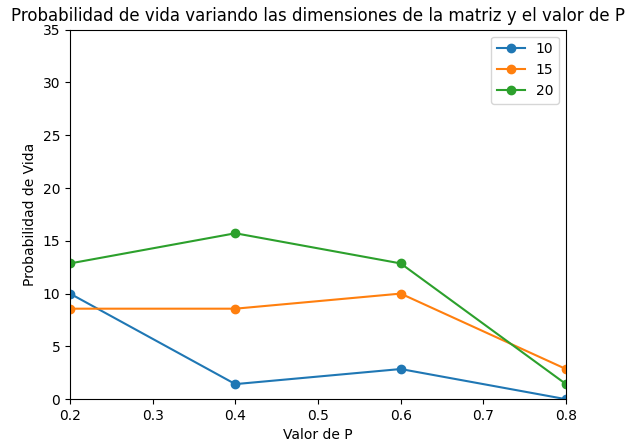
\includegraphics[width=140mm]{prob.png} 
    \caption{Probabilidad de que la matriz contenga vida después de 50 iteraciones, cada experimento se repitió 30 veces.}
    \label{prob}
\end{figure}
\begin{figure} 
    \centering
    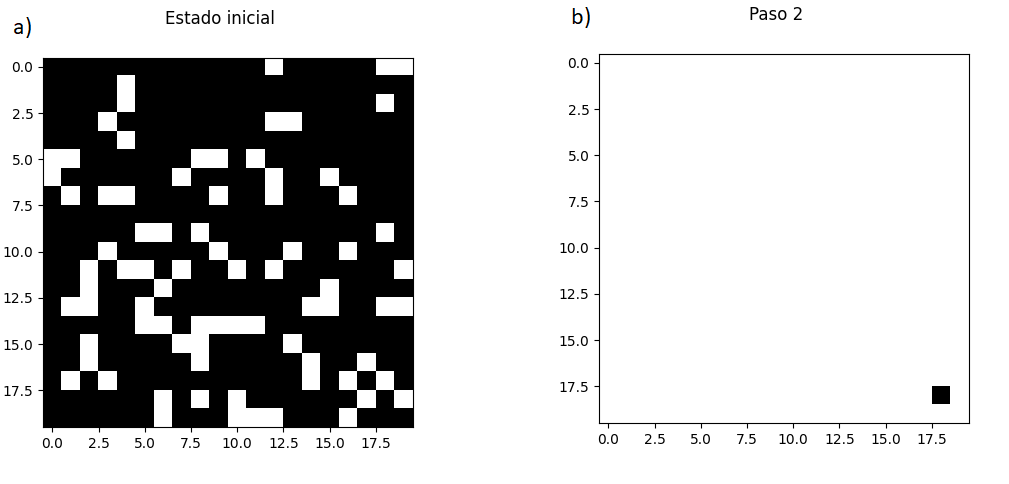
\includegraphics[width=140mm]{p0.4.png} 
    \caption{a)Estado inicial de una matriz cuando $p=0.8$ y $num=400$, se observa una saturación de las celdas que provoca vecindades igualmente saturadas por lo que la vida acaba a las pocas iteraciones. b)Paso 2 de la simulación, la vida es casi nula.}
    \label{p0.8}
\end{figure}

La generación de vida a partir de la colocación de semillas aleatorias se presenta en la figura \ref{semillas}. El propósito de esta simulación es evaluar el crecimiento de las semillas que no tocaron las fronteras de la estructura, la variación entre los tamaños de estos crecimientos van desde un elemento hasta 17 elementos para la semilla de tipo 10. Los mayores crecimientos tienen cuando menos un extremo ubicado en la parte central de la matriz (semilla 13,10 y 3). 
\begin{figure} 
    \centering
    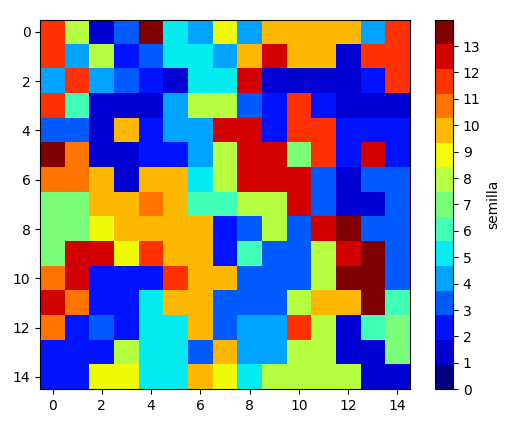
\includegraphics[width=140mm]{semillas.png} 
    \caption{Estado final de una matriz donde se sembraron semillas con valores de $1$ a $14$ de manera aleatoria al inicio de la simulación, el mayor crecimiento observado se presenta para la semilla $10$ con una cobertura de $17$ elementos.}
    \label{semillas}
\end{figure}

\begin{figure}[] 
    \centering
    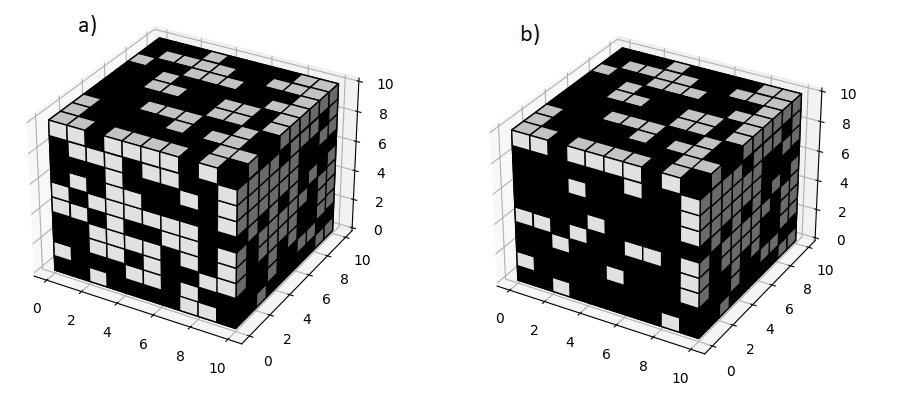
\includegraphics[width=140mm]{3d.png} 
    \caption{Simulación de un autómata en 3 dimensiones $p=0.5$ elimina elementos que en sus vecindades tenga más de 5 elementos vivos. a)Inicio de la simulación,elementos vivos=515, b) Final de la simulación,elementos vivos=205.}
    \label{3d}
\end{figure}
En la figura \ref{3d} se presenta el paso inicial y final de un autómata celular en tres dimensiones que sigue la lógica presentada en la sección 3.3. Para esta simulación $p$=$0.5$ para una matriz tridimensional de $10*10*10$ elementos. El número inicial de elementos vivos es de 515, después de 3000 iteraciones pseudoaleatorias quedaron vivos 205 elementos. 

\section{Conclusiones.}
 Las simulaciones pseudoaleatorias son herramientas poderosas que, como un primer acercamiento, nos dan la oportunidad de observar como podrían ocurrir algunos crecimientos en las estructuras. En este trabajo el valor de $p$ toma gran importancia, en otras palabras, nos indica la saturación que tendremos en el sistema y por tanto las interacciones que pueden ocurrir dentro del sistema.
\bibliography{simu}
\bibliographystyle{plainnat}
\end{document}



